% !TEX root = pfc.tex

De acordo com \cite{dnit:2011:online}, Departamento Nacional de Infra-Estrutura de Transportes, a contagem volumétrica consiste em quantificar o volume de veículos que trafegam por um determinado trecho da rodovia, durante um intervalo de tempo definido. A contagem de veículos é importante para o cumprimento de diversas finalidades, dentre elas: planejamento do sistema rodoviário, estabelecimento de tendências de tráfego futuro, determinação do volume de viagens de forma a proporcionar justificativa econômica aos investimentos programados, avaliação do fluxo existente de tráfego em relação ao sistema rodoviário atual, planejamento e justificativa do policiamento, realização de análise estatística de acidentes, estudos de localização de postos de pesagem, socorro médico emergencial, entre outros.

O volume de veículos, obtido através da contagem, pode ser classificado como \citep{goldner:2009:misc}:

\begin{itemize}
  \item \textbf{Volume de tráfego}: quantidade de veículos em tráfego na seção de uma via, em um período de tempo definido;
  \item \textbf{AADT} ou \textbf{VMDA}: volume médio diário de veículos durante o ano, ou seja, a somatória anual, dividido por 365;
  \item \textbf{ADT} ou \textbf{VMD}: volume diário do tráfego ou volume médio diário. Também é usado para intervalos de tempo diferentes, representando o volume total durante dado período, dividido pela quantidade de dias do período. Assim tem-se:
  \begin{itemize}
    \item \textbf{VMDm}: volume médio diário mensal. Número total de veículos em um mês, dividido pelo número de dias do mês;
    \item \textbf{VMDs}: volume médio diário semanal. Número total de veículos em uma semana, dividido por 7. É sempre acompanhado pelo nome do mês a que se refere;
    \item \textbf{VMDd}: Volume médio diário em um dia de semana. Deve ser sempre acompanhado pela indicação do dia de semana e do mês correspondente;
  \end{itemize}
  \item \textbf{Composição do tráfego}: porcentagem dos diferentes tipos de veículos que compõem o tráfego, por exemplo, automóveis, caminhões, ônibus e motos;
  \item \textbf{Volume abreviado}: volume do fluxo de um período menor do que 1 hora;
  \item \textbf{Variações do volume de tráfego}: mudanças no volume em um determinado período, divididas em: variações sazonais ou mensais ao longo do ano; variações diárias ao longo da semana; variações horárias ao longo do dia; e variações dentro da hora.
\end{itemize}

\cite{goldner:2009:misc} define dois métodos de contagem: \textbf{manual} e \textbf{mecânica}. A contagem manual utiliza recursos humanos, ou seja, pesquisadores observam o fluxo de veículos e manualmente fazem suas anotações. Esse procedimento é vantajoso pela precisão e variedade nas informações de tráfego obtidas, como tipo e tamanho dos veículos, além de proporcionar flexibilidade, simplicidade e rapidez de execução. No entanto, é um método com limitações de cobertura e de alto custo. A contagem mecânica utiliza detectores de tráfego de instalações permanente ou móvel. Possui algumas vantagens, dentre elas: baixo custo operacional, grande amplitude de tempo de cobertura e boa precisão. Por outro lado não fornecesse muitas informações e demanda investimento inicial alto.

A classificação feita por \cite{goldner:2009:misc} peca ao usar o termo contagem mecânica para caracterizar métodos não manuais. Grande parte dos equipamentos de contagem volumétrica são dispositivos eletrônicos, por exemplo sensores micro-ondas, ultra-sônicos e piezoelétricos, descaracterizando o uso dessa nomenclatura. Até mesmo o tubo pneumático, que pode ser considerado um dispositivo mecânico, utiliza sinais elétricos para transmissão dos dados. Por esse motivo, será adotado o termo \textbf{contagem automática} para descrever os métodos de contagem que não dependem diretamente da participação humana durante o processo de obtenção dos dados.

Por sua vez, os métodos automáticos de contagem podem ser classificados como \textbf{invasivos} e \textbf{não-invasivos}. Os métodos invasivos necessitam de instalações junto ou sob a camada asfáltica. Já os métodos não-invasivos não modificam a estrutura da via, com instalações acima ou às margens da faixa de tráfego \citep{goldner:2009:misc}.

Nas seções seguintes são apresentados alguns equipamentos automáticos de contagem volumétrica, descritos em \cite{goldner:2009:misc}, \cite{almeida:2010:masther} e \cite{dnit:2011:online}, bem como algumas aplicações de visão computacional inseridas na área de Engenharia de Transporte.

\section{Tecnologias detectoras de veículos} % (fold)
\label{sec:tecnologias_detectoras_de_ve_culos}

Atualmente existem diversas tecnologias de sensores capazes de efetuar a detecção de veículos \citep{minnesota1997field}. A Tabela \ref{tab:tecnologias_vantagens_desvantagens} lista grande parte delas, apresentando vantagens e desvantagens para cada uma \citep{aguiar2008thesis}. Nas subseções a seguir alguns sensores que utilizam essas tecnologias são detalhados.

\LTXtable{\textwidth}{advantages_disadvantages}

\subsection{Detector de laço indutivo} % (fold)
\label{sub:detectores_de_la_os_indutivos}

São os sensores mais utilizados para a coleta de dados de tráfego. É composto basicamente por um circuito elétrico oscilador, uma unidade eletrônica de processamento, cabos de transmissão e o laço indutivo propriamente dito, que é formado por uma ou mais voltas de um cabo isolado instalado sob o pavimento da via (Figura \ref{fig:laco_indutivo}), caracterizando-o como equipamento invasivo.

\begin{figure}[ht]
  \begin{center}
    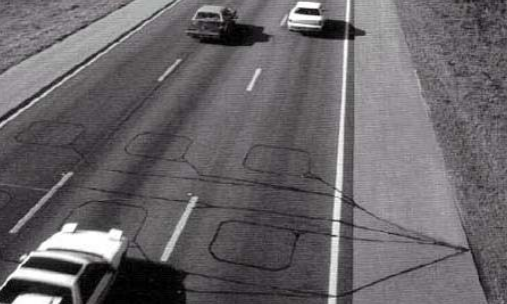
\includegraphics[scale=0.6]{imgs/laco_indutivo.png}
  \end{center}
  \caption{Seis laços indutivos instalado em uma rodovia, dois por faixa \citep{goldner:2009:misc}.}
  \label{fig:laco_indutivo}
\end{figure}

O laço funciona como indutor de um circuito oscilador de frequência fixa, normalmente entre 10 KHz e 200 KHz. Quando objetos de metal transitam nas proximidades do equipamento instalado no solo, acontece uma interação entre os campos magnéticos induzidos no laço e no objeto metálico, que normalmente é um veículo, provocando variações na indutância do laço e, portanto, variações na frequência de oscilação do circuito ressonante. A presença de um veículo na região do laço provoca um aumento na frequência de oscilação do circuito, comportamento que é interpretado pela unidade de processamento capaz de realizar a contagem.

Cada veículo que passa pelo laço indutivo possui um perfil magnético característico que depende de vários fatores, dentre eles, seu tamanho, formato, condutividade e orientação em relação ao laço. Isso possibilita, além da contagem, realizar uma classificação veicular através de métodos de clusterização por redes neurais, como descrito em \citep{almeida:2010:masther}.

A vantagem de se usar laços indutivos para monitoramento é o bom funcionamento na captura de dados básicos do tráfego, como volume e velocidade, além de apresentar baixo custo se comparado à equipamentos não-invasivos. Por outro lado, o processo de instalação do equipamento junto ao solo gera a paralisação no tráfego local e muitas vezes causa transtornos no trânsito.

% section detectores_de_la_os_indutivos (end)

\subsection{Tubo pneumático} % (fold)
\label{sub:tubo_pneum_tico}

Os sensores de contagem volumétrica por tubo pneumático funcionam a partir da pressão exercida pelos pneus de um veículo assim que passam sobre o tubo de borracha. A massa de ar é então deslocada ao longo do tubo até o ponto de conversão, onde um interruptor converte o sinal pneumático em sinal elétrico, para que esse possa ser transmitido a um \textit{software} de análise ou a um contador.

O tubo é instalado sobre a via, perpendicular à direção do fluxo do tráfego, caracterizando-se como um equipamento invasivo. É normalmente utilizado para contagem de tráfego em períodos curtos, classificação dos veículos por número de eixos e espaçamento, medição de velocidade e pesquisas acadêmicas.

Apesar de ser a primeira tecnologia de detecção de tráfego, inventada em 1920, é ainda muito utilizada devido ao baixo custo e a simples instalação e operação. No entanto, o equipamento é impreciso na contagem de caminhões ou ônibus muito largos, além de apresentar baixa durabilidade e sensibilidade à temperatura.

% section tubo_pneum_tico (end)

\subsection{Sensor magnético} % (fold)
\label{sub:sensores_magn_ticos}

O princípio de funcionamentos dos sensores magnéticos é baseado em variações das linhas de fluxo do campo magnético terrestre. Tal efeito é conhecido como anomalia magnética, causada pela aproximação de objetos metálicos (veículos) da área de cobertura do sensor. Por indução eletromagnética, variações de tensão são geradas e posteriormente amplificadas, digitalizadas e finalmente transmitidas ao controlador eletrônico que realiza a contagem.

São utilizados para medir volume, direção, presença e velocidade dos veículos. Podem ser divididos em dois tipos: os magnetômetros de indução, que se baseiam em mudanças nas linhas de fluxo do campo magnético devido ao movimento, não detectam veículos parados na via; e os magnetômetros de eixo duplo, que detectam mudanças nos componentes horizontais e verticais do campo magnético terrestre de acordo com a densidade do metal do veículo, e são capazes de identificar objetos em movimento ou parados.

 A utilização destes sensores é vantajosa devido a pouca sensibilidade à temperatura ambiente e ao tráfego intenso. Suas desvantagens são a pequena zona de detecção, a dificuldade em considerar veículos parados e a sua característica de instalação invasiva, fazendo-se necessárias paralizações do tráfego e interferências na camada asfáltica.

% section sensores_magn_ticos (end)

\subsection{Sensor piezoelétrico} % (fold)
\label{sub:sensores_piezoel_tricos}

Um material piezoelétrico é capaz de converter energia cinética em energia elétrica. Esses materiais geram uma tensão quando submetidos a choques mecânicos ou vibrações. Portanto, quando um veículo passa sobre um detector, o sensor gera uma tensão proporcional ao peso do veículo. É construído a partir de um cabo piezoelétrico do tipo coaxial, com um núcleo de metal, seguido pelo material piezoelétrico e uma camada externa de metal, como ilustrado na Figura \ref{fig:piezoeletrico}.

\begin{figure}[ht]
  \begin{center}
    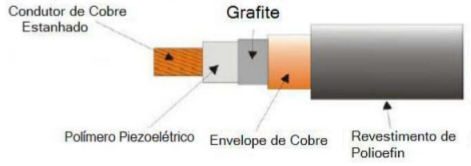
\includegraphics[scale=0.6]{imgs/piezoeletrico.png}
  \end{center}
  \caption{Representação esquemática de um cabo piezoelétrico \citep{goldner:2009:misc}.}
  \label{fig:piezoeletrico}
\end{figure}

Devido a sua grande precisão, esse tipo de sensor é capaz de medir volume do tráfego, velocidade, peso e ainda classificar os veículos baseado no espaçamento e contagem de eixos. Sua instalação é feita junto à via, caracterizando-o como invasivo, e não é recomendado em solos irregulares. Apresenta alto custo se comparado a outros equipamentos invasivos, mas em contrapartida são mais precisos e adquirem informações mais completas.

% section sensores_piezoel_tricos (end)

\subsection{Câmera de vídeo} % (fold)
\label{sub:c_mera_de_v_deo}

As câmeras de vídeo são utilizadas no monitoramento do tráfego, na maioria das vezes, como uma simples ferramenta de vigilância urbana, com capacidades de transmissão e gravação de imagens. Nesse cenário, as imagens devem ser interpretadas por um operador humano, que tem a função de extrair dados de tráfego. Com o avanço das áreas de processamento digital de imagens e visão computacional, surgiram diversos sistemas de gerenciamento do tráfego capazes de extrair automaticamente informações de tráfego importantes, como velocidade, volume, presença, ocupação, densidade, movimentos de conversão, mudança de faixa, aceleração, classificação de veículos e outros \citep{martinsky:2007:masther,feitosa:2012:masther}.

Um sistema inteligente de processamento de imagens de vídeo consiste em uma ou mais câmeras, um \textit{hardware}\footnote{Parte física de computadores ou quaisquer equipamentos eletrônicos.} para digitalização e processamento e um \textit{software} para interpretação e conversão de imagens em dados de tráfego, numéricos ou simbólicos. Segundo \cite{feitosa:2012:masther}, esse tipo de sistema pode, com apenas uma câmera, substituir vários equipamentos invasivos, como laços indutivos, e proporcionar detecção de veículos em múltiplas faixas com menores custos de manutenção.

Dentre as vantagens de uso de câmeras está a instalação, que é totalmente não-invasiva e não gera qualquer tipo de transtorno ao trânsito. Uma vez capturadas, as imagens do tráfego podem ser analisadas posteriormente por profissionais capazes de, por exemplo, realizar a contagem volumétrica manual ou periciar um acidente. Mudanças naturais na cena, como chuvas, tempo nublado, o dia e a noite, podem interferir na visibilidade, dificultando tanto a interpretação humana quanto o processamento digital por visão computacional. Deslocamentos indesejados da câmera e problemas de oclusão também são comuns.

% section c_mera_de_v_deo (end)

\subsection{Sensores micro-ondas} % (fold)
\label{sub:radar_por_microondas}

Esse tipo de equipamento transmite radiação de micro-ondas de baixa energia na direção de uma área do pavimento utilizando uma antena localizada na parte superior do radar. Quando um veículo atravessa um feixe, uma parte dessa energia é refletida de volta para o detector, também localizado na parte superior do radar, e dados como velocidade e presença são calculados por um controlador. A Figura \ref{fig:microondas} ilustra a configuração mais comum de um sistema de monitoramento baseado em sensores micro-ondas.

\begin{figure}[ht]
  \begin{center}
    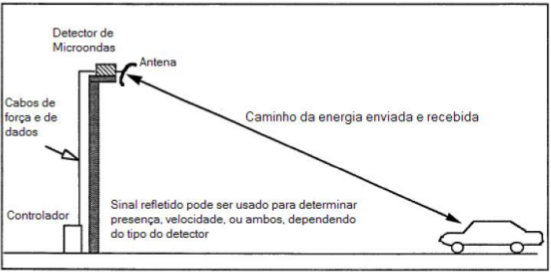
\includegraphics[scale=.6]{imgs/microondas.png}
  \end{center}
  \caption{Esquema ilustrativo da arquitetura de um sistema de monitoramento do tráfego baseado em sensores micro-ondas \citep{goldner:2009:misc}.}
  \label{fig:microondas}
\end{figure}

Esses sensores podem ser de dois tipos:

\begin{itemize}
  \item \textbf{Doppler}: mede a presença de um veículo em função do movimento relativo entre uma fonte sonora e seu receptor e que, por efeito \textit{Doppler}, varia a frequência recebida na volta. Como é um método baseado em movimento, não considera veículos parados ou em regime de ``anda-pára''.
  \item \textbf{Radar}: utiliza um sinal de frequência ou fase modulada para calcular o atraso de tempo da onda refletida, obtendo a distância do veículo. Nesse método é possível detectar a presença de veículos parados, além de medir velocidade, monitorar filas e ocupação.
\end{itemize}

Os sensores micro-ondas são não-invasivos e não interferem no tráfego de veículos no processo de instalação. Geralmente não apresentam sensibilidade em más condições climáticas e podem ser construídos para suportar múltiplas pistas. No entanto, um dos tipos não é capaz de detectar veículos parados.

% section radar_por_microondas (end)

\subsection{Sensores ultrassônicos} % (fold)
\label{sec:sensores_ultrass_nicos}

Esses detectores transmitem ondas de pressão de energia sonora acima da frequência audível humana, que é de 20 KHz. Estas ondas sonoras refletem no pavimento ou no veículo, são captadas por um receptor e processadas para fornecer informações de passagem e presença de veículos. A montagem não-invasiva do equipamento pode ser feita acima ou ao lado da via, como ilustra a Figura \ref{fig:ultrassonico}.

\begin{figure}[ht]
  \begin{center}
    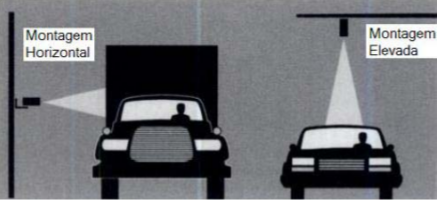
\includegraphics[scale=.65]{imgs/ultrassonico.png}
  \end{center}
  \caption{Tipos de montagem para um sensor ultrassônico \citep{goldner:2009:misc}.}
  \label{fig:ultrassonico}
\end{figure}

Existem dois tipos de sensores ultrassônicos:

\begin{itemize}
  \item \textbf{Pulso ultrassônico}: são emitidos pulsos de energia com largura e período conhecidos. Se o tempo do pulso refletido for menor que o valor conhecido, a presença do veículo é acusada, fornecendo informações de altura, largura, ocupação, volume e classificação.
  \item \textbf{Onda ultrassônica contínua}: usam o princípio  de \textit{Doppler}, que leva em conta a variação da frequência causada pela velocidade relativa entre onda emitida e refletida, para determinar a presença, volume e velocidade veicular.
\end{itemize}

O uso de sensores ultrassônicos é vantajoso pois a instalação é não-invasiva e pode monitorar mais de uma pista ao mesmo tempo. Como desvantagem, as mudanças de temperatura e ventanias podem afetar o seu desempenho.

% section sensores_ultrass_nicos (end)

% section tecnologias_detectoras_de_ve_culos (end)


\section{Aplicações de Visão Computacional} % (fold)
\label{sec:aplica_es_de_vis_o_computacional}

Com o desenvolvimento de pesquisas na área de processamento de imagens digitais nos últimos tempos, impulsionado pelas facilidades de implementação de aplicações de visão computacional utilizando a biblioteca OpenCV \citep{opencv_library}, cada vez mais trabalhos de monitoramento do tráfego que utilizam visão computacional são publicados. A seguir, uma breve revisão bibliográfica de projetos de Engenharia de Transporte que utilizam conceitos de visão computacional.

% \subsection{Direção autônoma de veículo inteligente} % (fold)
% \label{sub:dire_o_aut_noma_de_ve_culo_inteligente}

% \cite{thrun:2006:article}
%TODO: importante por causa do Guilherme

% % subsection dire_o_aut_noma_de_ve_culo_inteligente (end)

% \subsection{Detecção de placa de veículos} % (fold)
% \label{sub:detec_o_de_placa_de_ve_culos}

% \cite{martinsky:2007:masther}

% % subsection detec_o_de_placa_de_ve_culos (end)

\subsection{Contagem volumétrica utilizando dispositivos móveis} % (fold)
\label{sub:contagem_volum_trica_utilizando_dispositivos_m_veis}

\cite{feitosa:2012:masther} propõe em sua Tese de Mestrado em Ciência da Computação pela UFG - Universidade Federal de Goiás, um método para contagem volumétrica de veículos baseado em visão computacional. A pesquisa é focada em otimização de algoritmos de processamento de imagens para execução em dispositivos móveis.

Alguns requisitos são estabelecidos nesse trabalho: as imagens são capturadas da lateral de uma via, com uma câmera fixada em uma baixa altura, identificando e contando veículos que trafegam em ambas as direções; as imagens utilizadas são de baixa resolução; e o processo de contagem é realizado em tempo real.

Apesar de o objetivo do projeto ser a contagem volumétrica via dispositivos móveis, o estudo inicial das técnicas de processamento de imagem e visão computacional é feito em um \textit{laptop}\footnote{Computador portátil, que no Brasil também é conhecido como \textit{notebook}}. A metodologia adotada pode ser dividida em seis etapas principais. São elas:

\begin{enumerate}
  \item \textbf{Entrada de dados}: os \textit{frames}\footnote{Cada um dos quadros de um vídeo.} do vídeo são disponilizados em tempo real ou por um arquivo em disco, que foi gravado anteriormente.
  \item \textbf{Pré-processamento de imagem}: conversão para escala de cinza, caso ainda não esteja nesse formato; equalização do histograma; e suavização da imagem por filtragem linear.
  \item \textbf{Reconhecimento da imagem referência de fundo}: obtenção de um modelo adaptativo da imagem de fundo da cena, utilizando um método de rápido processamento.
  \item \textbf{Definição da área de movimento}: determinação da região da cena com maior movimentação que, provavelmente, é a área de tráfego de veículos. Essa região de interesse também elimina movimentações indesejadas, como por exemplo, o movimento da vegetação.
  \item \textbf{Segmentação de objetos}: subtrai a imagem referência de fundo do \textit{frame} corrente, segmentando os objetos de interesse. Também descarta objetos sem interesse.
  \item \textbf{Acompanhamento de objetos segmentados}: rastreamento dos objetos segmentados ao longo dos quadros, evitando que o mesmo seja contado mais de uma vez.
\end{enumerate}

O método proposto foi implementado em forma de aplicativo na linguagem Java, utilizando a biblioteca de processamento de imagens JavaCV, que utiliza a maior parte das funções da OpenCV \citep{opencv_library}. Como o trabalho de \cite{feitosa:2012:masther} tem por objetivo a execução em dispositivos móveis, o desempenho do algoritmo é um fator determinante. Por isso, foi necessário que alguns algoritmos de processamento de imagens, já existentes na OpenCV, fossem reimplementados com foco em velocidade de execução, o que elevou muito a complexidade do código. Na etapa de reconhecimento da imagem referência de fundo, por exemplo, seria muito mais simples, do ponto de vista de desenvolvimento, utilizar as funções de subtração de \textit{backgroud} já implementadas na OpenCV. No entanto, por ser um método mais completo e complexo, acarretaria em menor desempenho de execução se comparado à implementação de \cite{feitosa:2012:masther}.

Os testes foram realizados a partir de 15 amostras de vídeos, sendo 14 com resolução $640\times 480$ e apenas 1 com resolução $320\times 240$, e duração média de 09:30 minutos. Para avaliar o desempenho do método, num primeiro momento foi feita uma contagem volumétrica manual dos veículos em cada amostra, para que assim o percentual de acerto do método automático, executado no \textit{laptop}, fosse calculado. Além disso, o tempo de execução de cada amostra foi medido.

Em seguida, o aplicativo desenvolvido em Java foi adaptado para ser executado por um dispositivo móvel com sistema operacional Android. Os mesmos testes foram realizados para as 15 amostras e o percentual de acerto permaneceu o mesmo, resultado esperado tendo em vista que os algoritmos de processamento de imagem e visão computacional não mudaram. Nesse novo cenário, o tempo de execução também foi medido. A Tabela \ref{tab:feitosa} lista as medições de cinco amostras.


\begin{table}[ht]
  \caption{Comparação entre resultados de tempo de execução do método pelo \textit{laptop} e celular \citep{feitosa:2012:masther}.}
  \label{tab:feitosa}
  \begin{center}
    \begin{tabular}{ccccc}
    \toprule
    \textbf{Amostra} & \textbf{\% acerto} & \textbf{Duração} & \textbf{Tempo celular} & \textbf{Tempo \textit{laptop}}\\
    \midrule
      1 & 90,58 & 00:15:08 & 01:00:56 & 00:03:54\\
      2 & 92,45 & 00:05:15 & 00:19:55 & 00:01:36\\
      3 & 91,30 & 00:02:44 & 00:11:55 & 00:00:27\\
      4 & 98,15 & 00:10:18 & 00:48:18 & 00:03:39\\
      5 & 97,71 & 00:13:07 & 01:09:27 & 00:03:48\\
    \bottomrule
    \end{tabular}
  \end{center}
\end{table}

Os percentual de acerto obtido nas contagens foi satisfatórios e o aplicativo desenvolvido para executar em um \textit{laptop} foi adaptado e portado para um dispositivo móvel Android com sucesso. No entanto, o tempo de execução do método no dispositivo móvel não foi satisfatório, inviabilizando que essa aplicação funcione em tempo real.

% subsection contagem_volum_trica_utilizando_dispositivos_m_veis (end)

% section aplica_es_de_vis_o_computacional (end)